\documentclass{report}

\title{Mécatro: Rapport d'automatique}
\author{Groupe 7: Royer Jules, Simon Noah-Luc, Colin Matthieu, Bourderioux Armand}

\date{}

\usepackage[T1]{fontenc}
\usepackage{lmodern}

\usepackage[margin=0.7in]{geometry}

\usepackage{amssymb}
\usepackage{gensymb}
\usepackage{mathrsfs}

\usepackage{amsmath}
\usepackage{mathtools}

\usepackage{graphicx}
\usepackage{caption}
\usepackage{subcaption}
\usepackage{float}

\usepackage[parfill]{parskip}

\preto{\subsection}{\Needspace{5\baselineskip}}
\preto{\section}{\Needspace{5\baselineskip}}

\hyphenpenalty=10000

\usepackage{listings}
\usepackage{pxfonts}

\usepackage{biblatex}
\addbibresource{bibliography.bib}

\usepackage{blindtext}

\usepackage{hyperref}

\begin{document}

\maketitle

\tableofcontents

\chapter{Introduction}
Le but de la partie automatique du projet de mécatronique est de créer un contrôleur
pour un robot "bolide" suiveur de ligne. Le contrôleur a d'abord été créé théoriquement
dans le logiciel Matlab et testé sur un modèle de simulation Simulink, puis il a été
implémenté informatiquement en Arduino afin d'être embarqué dans le robot.

\chapter{Création du contrôleur théorique}

\paragraph{Contrôle d'un mouvement rectiligne uniforme}

En reprenant les notations et la modélisation du document "Equations de la dynamique du Segway",
les équations de la dynamique sous forme d'état sont (on négligera toutes les perturbations):

\begin{equation*}
    \begin{cases}
        \dot{p} = u \\
        \dot{u} = \frac{1}{\beta}\big( \frac{1}{\rho}kI^{+} - m_bdv^2 \big) \\
        \dot{\psi} = v \\
        \dot{v} = \frac{1}{\gamma}\big( \frac{lk}{2\rho}I^{-} + m_bduv \big) \\
        \dot{I^{+}} = \frac{U^{+}}{L} - \frac{R}{L}I^{+} - \frac{2k}{L\rho}u \\
        \dot{I^{-}} = \frac{U^{-}}{L} - \frac{R}{L}I^{-} - \frac{kl}{L\rho}v \\
        \dot{y} = u\sin\psi \\
    \end{cases}
\end{equation*}

Les entrées sont $U^{+}$, $U^{-}$.

Les sorties mesurées sont:

\begin{equation*}
    \begin{cases}
        \delta \delta \phi^{+} = \delta \phi_{right} + \delta \phi_{left} = \frac{2}{\rho}p \\
        \delta \delta \phi^{-} = \delta \phi_{right} + \delta \phi_{left} = \frac{l}{\rho}\psi \\
        c_{LF} = \frac{y}{\cos\psi} \approx y \\
    \end{cases}
\end{equation*}

Où on a défini:

\begin{itemize}
    \item $p$ la distance curviligne parcourue par le robot le long de sa trajectoire.
    Celle-ci doit figurer dans l'état pour mesurer les angles cumulés.
    \item $u$ sa vitesse longitudinale.
    \item $\psi$ l'angle entre l'axe horizontal $x$ et la direction du robot.
    \item $I^{-} = I_{right} - I_{left}$ la somme des courants des moteurs.
    \item $I^{-} = I_{right} - I_{left}$ la différence des courants.
    \item $U^{+} = U_{right} + U_{left}$ la somme des tensions aux bornes des moteurs.
    \item $U^{-} = U_{right} - U_{left}$ la différence des tensions.
    \item $\beta = M + \frac{2I^{w}_{y}}{\rho^2}$
    \item $\gamma = I_{\psi} + m_bd^2$
    \item $\phi^{+}$ la somme des angles des roues. Posons $\alpha = \frac{2}{\rho}$.
    \item $\phi^{-}$ la différence des angles des roues. Posons  $\eta = \frac{l}{\rho}$.
    \item $c_{LF}$ la mesure de l'écart entre le point A et la ligne (approximation en MRU horizontal).
\end{itemize}


\begin{figure}[h]  % Placement "here"
    \centering
    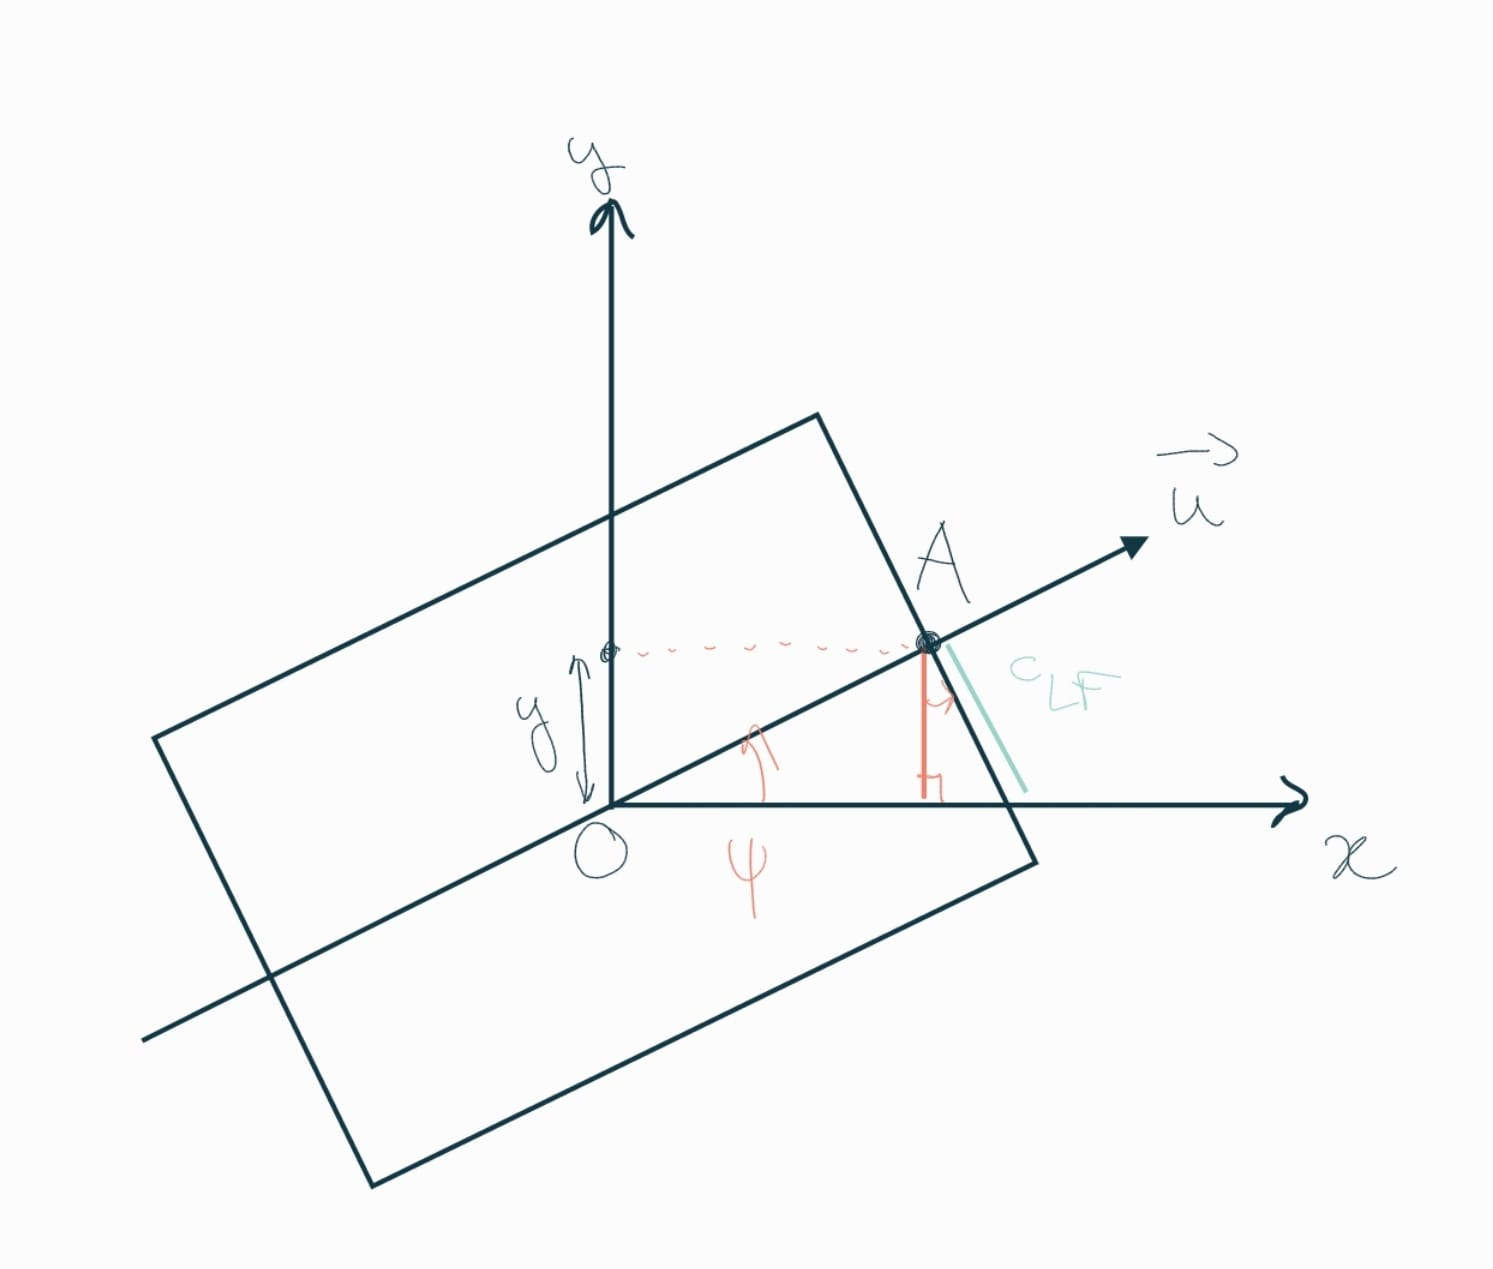
\includegraphics[width=0.5\textwidth]{figures/cLF_schema.jpg}
    \caption{Ecart à la ligne dans l'hypothèse d'un faible angle.}
\end{figure}


\paragraph{Recherche des trajectoires d'équilibre}

Notre trajectoire d'équilibre du mouvement rectiligne uniforme 
est caractérisée par le système:

\begin{equation*}
    \begin{cases}
        u_0 = \overline{u} \\
        0 = \frac{1}{\beta}\big( \frac{1}{\rho}k\overline{I^{+}} - m_bd\overline{v}^2 \big) \\
        0 = \overline{v} \\
        0 = \frac{1}{\gamma}\big( \frac{lk}{2\rho}I^{-} + m_bd\overline{u}\overline{v} \big) \\
        0 = \frac{\overline{U^{+}}}{L} - \frac{R}{L}\overline{I^{+}} - \frac{2k}{L\rho}\overline{u} \\
        0 = \frac{\overline{U^{-}}}{L} - \frac{R}{L}\overline{I^{-}} - \frac{kl}{L\rho}\overline{v} \\
        0 = \overline{u}\sin\overline{\psi} \\
    \end{cases}
\end{equation*}

Avec les sorties linéarisées:

\begin{equation*}
    \begin{cases}
        \delta \phi^{+} = \alpha \delta p \\
        \delta \phi^{-} = \eta \delta \psi \\
        \delta c_{LF} = \delta y \\
    \end{cases}
\end{equation*}

Ce qui donne comme trajectoire d'équilibre 
\begin{equation*}
    \begin{cases}
        \underline{x} = \big(\overline{p}=u_0t, \overline{u}=0, \overline{\psi}=\psi_0=0, 
        \overline{v}=0, \overline{I^{\pm}}=0, \overline{y}=0 \big) \\
        \underline{e} = \big( \overline{U^{+}}=\frac{2k}{\rho} u_0, \overline{U^{-}}=0 \big)
    \end{cases}
\end{equation*}

\paragraph{Linéarisé autour de l'équilibre}

\begin{equation*}
    \begin{cases}
        \delta{\dot p} = \delta u \\
        \delta{\dot u} = \frac{1}{\beta}\frac{1}{\rho}k\delta I^{+} \\
        \delta{\dot \psi} = \delta v \\
        \delta{\dot v} = \frac{1}{\gamma}\big( \frac{lk}{2\rho}\delta I^{-} + m_bd u_0 \delta v \big) \\
        \delta{\dot I^{+}} = \frac{\delta U^{+}}{L} - \frac{R}{L}\delta I^{+} - \frac{2k}{L\rho}\delta u \\
        \delta{\dot I^{-}} = \frac{\delta U^{-}}{L} - \frac{R}{L}\delta I^{-} - \frac{kl}{L\rho}\delta v \\
        \dot{y} = u_0\cos\psi_0 \delta \psi + \delta u \sin\psi_0 = u_0 \delta \psi \\
    \end{cases}
\end{equation*}

\begin{figure}[h]  % Placement "here"
    \centering
    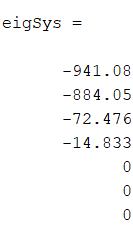
\includegraphics[width=0.2\textwidth]{figures/eigSys.png}
    \caption{Valeurs propres du système linéarisé.}
\end{figure}

Les valeurs propres obtenus sont négatives. Celles qui sont nulles sont
dûes au fait que certaines variables d'état sont redondantes: $p$, $y$,
donc le système reste stable.

% Il est étrange que les 2 valeurs propres rapides soient différentes, car
% celles de $I_l, I_r$ sont égales et que le changement en $I^+,I^-$.

\paragraph{Simplifications par perturbations singulières}

Les intensités de courant ont un transitoire bien plus rapide que
ceux des grandeurs mécaniques (leurs valeurs propres $\frac{R}{L}$ sont bien supérieures aux autres).

On applique la méthode des perturbations singulières à:
\begin{equation*}
    \begin{cases}
        L\dot{I^{+}} = U^{+} - RI^{+} - \frac{2k}{\rho}u \\
        L\dot{I^{-}} = U^{-} - RI^{-} - \frac{kl}{\rho}v \\
    \end{cases}
\end{equation*}

Avec $\varepsilon = L$ "très petit". En tout rigueur il faudrait introduire
$L_0$ pour adimensionner $\varepsilon$.

On obtient:

\begin{equation*}
    \begin{cases}
        I^{+} = \frac{1}{R} \big(U^{+} - \frac{2k}{\rho}u \big) \\
        I^{-} = \frac{1}{R} \big(U^{-} - \frac{kl}{\rho}v \big)\\
    \end{cases}
\end{equation*}

On vérifie la stabilité uniformément exponentielle de la branche d'équilibre avec :

\begin{equation*}
    \partial_{I^{\pm}}
    \begin{pmatrix}
        \frac{U^{+}}{L} - \frac{R}{L}I^{+} - \frac{2k}{L\rho}u  \\
        \frac{U^{-}}{L} - \frac{R}{L}I^{-} - \frac{kl}{L\rho}v  
    \end{pmatrix} \biggr\rvert_{I^{\pm} = f(\underline{x}, \underline{e})}
    = -\frac{R}{L}
    \begin{pmatrix}
        1 & 0 \\
        0 & 1
    \end{pmatrix}
\end{equation*}

La branche a donc comme valeurs propres des réels négatifs, donc est ue-stable.

\paragraph{Système lent simplifié}

\begin{equation*}
    \begin{cases}
        \delta{\dot p} = \delta u \\
        \delta{\dot u} = \underbrace{\frac{1}{\beta}\frac{k}{\rho}\frac{1}{R}}_{Q} \big( \delta U^+ - \frac{2k}{\rho}\delta u \big)\\
        \delta{\dot \psi} = \delta v \\
        \delta{\dot v} = \underbrace{\frac{1}{\gamma} m_bd u_0}_{b_1} \delta v + 
        \underbrace{\frac{1}{\gamma}\frac{lk}{2\rho}\frac{1}{R}}_{b_2}\big( \delta U^- - \frac{lk}{\rho}\delta v \big) \\
        \dot{y} = u_0\delta \psi        
    \end{cases}
\end{equation*}


\paragraph{Découplage en sous-système "Sum" et "Dif"}

On peut séparer le système global en 2 sous-systèmes indépendants.
Le premier, appelé "Sum", régit la dynamique du bolide
en ligne droite:

\begin{equation*}
    \text{Etat}
    \begin{cases}
        \delta{\dot p} = \delta u \\
        \delta{\dot u} = Q\big( \delta U^+ - \frac{2k}{\rho}\delta u \big)\\
    \end{cases}
    \text{Sorties}
    \begin{cases}
        \delta y_m^+ = \delta \phi^+        
    \end{cases}
\end{equation*}

Le second, appelé "Dif", régit la dynamique du bolide dans les virages:

\begin{equation*}
    \text{Etat}
    \begin{cases}
        \delta{\dot \psi} = \delta v \\
        \delta{\dot v} = b_1\delta v + b_2\big( \delta U^- - \frac{lk}{\rho}\delta v \big) \\
        \dot{y} = u_0\delta \psi        
    \end{cases}
    \text{Sorties}
    \begin{cases}
        \delta y_m^- = \delta \phi^- \\ 
        \delta c_{LF} = \delta y  
    \end{cases}
\end{equation*}

On obtient les valeurs propres suivantes:

\begin{figure}[h]  % Placement "here"
    \begin{subfigure}{.5\textwidth}
        \centering
        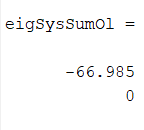
\includegraphics[width=0.2\textwidth]{figures/eigSysSumOl.png}        
      \end{subfigure}    
      \begin{subfigure}{.5\textwidth}
        \centering
        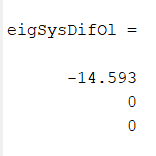
\includegraphics[width=0.2\textwidth]{figures/eigSysDifOl.png}
      \end{subfigure}    
      \caption{Valeurs propres des sous-systèmes linéarisés. 
      Environ égales aux plus lentes du linéarisé global.}
\end{figure}

\paragraph{Modélisation du contrôleur du sous-système "Sum"}

L'état étant de dimension 2, notre choix s'est porté sur un Proportionnel
- Dérivé permettant de contrôler $U^+$ avec $\phi^+$:

\begin{equation*}
    \delta{U^+} = h_1(\delta \phi^+_r - \delta \phi^+) 
    - h_2(\delta \dot{\phi}^+_r - \delta \dot{\phi}^+) \\     
    =h_1\alpha( \delta p_r - \delta p) 
    - h_2\alpha( \delta u_r - \delta u)
\end{equation*}
\begin{equation*}
    \text{En Laplace: }
    \underline{U^+} = \frac{-h_2s + h_1}{1}
    (\underline{\phi^+_r} -\underline{\phi^+})
\end{equation*}

Pour ajuster le comportement de notre système en boucle fermée, nous 
imposons le polynôme caractéristique de $A^+ = \partial_{\underline{x}^+} f$
où $f^+$ est la fonction de la dynamique de l'état $\underline{x}^+$:
\begin{equation*}
    \chi_{A^+ \text{ désiré}} = s^2 + 2\xi\omega_0 s + \omega_0^2
\end{equation*}

Où l'amortissement $\xi$ et la pulsation propre $\omega_0$ sont à ajuster.

En boucle fermée:

\begin{equation*}
    \begin{pmatrix}
        \delta{\dot p} \\
        \delta{\dot u} \\
    \end{pmatrix}
    =
    \underbrace{
    \begin{pmatrix}
        0 & 1 \\
        \underbrace{-Q\alpha h_1}_{a_1} & +\underbrace{Q(\alpha h_2 - \frac{2k}{\rho}}_{a_2})
    \end{pmatrix}
    }_{A^+}
    \begin{pmatrix}
        \delta{p} \\
        \delta{u} \\
    \end{pmatrix}
    +
    \begin{pmatrix}
        0 & 0 \\
        Q\alpha h_1 & -Q\alpha h_2
    \end{pmatrix}
    \begin{pmatrix}
        \delta{p_r} \\
        \delta{u_r} \\
    \end{pmatrix}
    \Rightarrow
    \chi_{A^+} = s^2 - a_2 - a_1
\end{equation*}


\begin{equation*}
    \text{Identification}
    \begin{cases}
        -a_2=2\xi \omega_2 \\
        -a_1 = \omega_0^2
    \end{cases}
    \Leftrightarrow
    \begin{cases}
        h_2 = \frac{1}{\alpha}\big( \frac{2\xi\omega_0}{-Q}+\frac{2k}{\rho})\\
        h_1 = \frac{\omega_0^2}{Q\alpha}
    \end{cases}
\end{equation*}

\paragraph{Modélisation du contrôleur du sous-système "Dif"}
Pour contrôler l'état de dimension 3, on a choisit un Proportionnel - Dérivé
sur la différence des angles cumulés $\phi^-$ 
et un proportionnel sur l'écart à la ligne $c_{LF}$ pour contrôler $U^-$:

\begin{equation*}
    \delta U^- = k_1(\delta \phi^-_r - \delta \phi^-)
    - k_2(\delta \dot{\phi}^-_r - \delta \dot{\phi}^-)
    + k_5(\delta c_{LFr} - \delta c_{LF}) \\
    = k_1 \eta(\delta \psi_r - \delta \psi^-)
    - k_2 \eta(\delta \dot{\psi}_r - \delta \dot{\psi}^-)
    + k_5(\delta y_r - \delta y) \\
\end{equation*}
\begin{equation*}
    \text{En Laplace: }
    \underline{U^-} = \frac{-k_2s + k_1}{1}
    (\underline{\phi}^-_r - \underline{\phi}^-)
    + \frac{k_5}{1}
    (\underline{c_{LFr}} - \underline{c_{LF}})    
\end{equation*}

Pour ajuster le comportement de notre système en boucle fermée, nous 
imposons:
\begin{equation*}
    \chi_{A^- \text{ désiré}} = s^3 + \sigma\sqrt{6}s^2 
    + \sigma^2\sqrt{6}s + \sigma^3 
\end{equation*}

En boucle fermée:

\begin{equation*}
    \begin{cases}
        \delta \dot{\psi} = \delta v \\
        \delta \dot{v} = \underbrace{-k_1b_2\eta\delta}_{c_1} \psi + 
        \underbrace{\big(b_1 + b_2k_2\eta - \frac{b_2kl}{\rho} \big)}_{c_2}\delta v 
        \underbrace{- b_2k_5}_{c_3} \delta y
    \end{cases}
\end{equation*}

On a

\begin{equation*}
    A^-=
    \begin{pmatrix}
        0 & 1 & 0 \\
        c_1 & c_2 & c_3 \\
        u_0 & 0 & 0 \\
    \end{pmatrix}
\end{equation*}
 On identifie
 \begin{equation*}
    \chi_{A^-} = s^3 - c_2s - c_1s - u_0c_3
    = s^3 + \sigma\sqrt{6}s^2 
    + \sigma^2\sqrt{6}s + \sigma^3 \\    
 \end{equation*}
 \begin{equation*}
    \Leftrightarrow
    \begin{cases}
        k_1 = \frac{1}{b_2\eta}\sigma^2\sqrt{6}  \\
        k_2 = \frac{1}{b_2\eta}\big(-\sigma\sqrt{6} - b_1 + b_2\frac{kl}{\rho} \big) \\
        k_5 = \frac{\sigma^3}{u_0b_3}  
    \end{cases}
 \end{equation*}

\paragraph{Approximation des contrôleurs avec des dérivées filtrées}

Pour le sous-système "Sum", le contrôleur en dérivée filtrée s'écrit:

\begin{equation*}
    \begin{cases}
        \dot{\eta} = \frac{\Delta \phi^+ - \eta}{\varepsilon}
        =  n_s\big(\Delta \phi^+ - \eta \big) 
        \text{ où } \Delta \phi^+ = \delta \phi^+_r - \delta \phi^+
        \text{ et } n_s = \frac{1}{\varepsilon} \\
        \delta{U^+} = h_1(1 - T_{ds}n_s)\Delta \phi^+ +
        h_1T_{ds}n_s\eta \text{ où } T_{ds} = \frac{h_2}{h_1} 
    \end{cases}
\end{equation*}

De même pour le sous-système "Dif":

\begin{equation*}
    \begin{cases}
        \dot{\eta} = \frac{\Delta \phi^- - \eta}{\varepsilon}
        =  n_d\big(\Delta \phi^- - \eta \big) 
        \text{ où } \Delta \phi^- = \delta \phi^-_r - \delta \phi^-
        \text{ et } n_d = \frac{1}{\varepsilon} \\
        \delta{U^-} = k_1(1 - T_{dd}n_d)\Delta \phi^- +
        k_1T_{dd}n_d\eta + k_5 \Delta c_{LF}\text{ où } T_{dd} = \frac{k_2}{k_1} \text{ et }
        \Delta c_{LF} = \delta c_{LFr} - \delta c_{LF}
    \end{cases}
\end{equation*}

\paragraph{Réponses fréquentielles des systèmes fermés modélisés 
en Matlab}

Pour le système "Sum", nous ne voulions pas trop accélérer la dynamique,
ainsi nous avons pris $\omega_0 = |\lambda^+|$ la valeur propre du système,
et l'amortissement $\xi = \frac{1}{\sqrt{2}}$, afin d'avoir en boucle fermée
(avec $n_s=150$):

\begin{figure}[h]  % Placement "here"
    \begin{subfigure}{.5\textwidth}
        \centering
        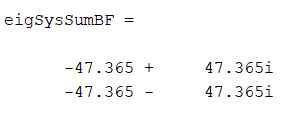
\includegraphics[width=0.8\textwidth]{figures/eigSysSumBF.png}        
      \end{subfigure}    
      \begin{subfigure}{.5\textwidth}
        \centering
        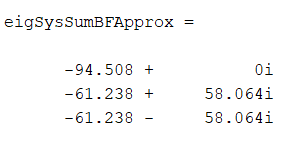
\includegraphics[width=0.8\textwidth]{figures/eigSysSumBFApprox.png}
      \end{subfigure}    
      \caption{Valeurs propres de "Sum" avec contrôleur PD, 
      (gauche: contrôleur idéal, droite: dérivée filtrée).
      Elles sont inférieures à celles en boucle ouverte.}
\end{figure}


\begin{figure}[h]  % Placement "here"
    \begin{subfigure}{.4\textwidth}
        \centering
        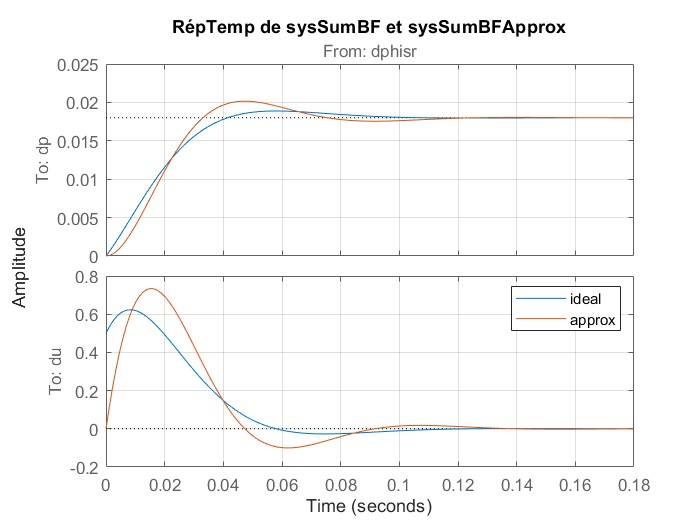
\includegraphics[width=\textwidth]{figures/reptempsumbf_approx.jpg}        
      \end{subfigure}    
      \begin{subfigure}{.6\textwidth}
        \centering
        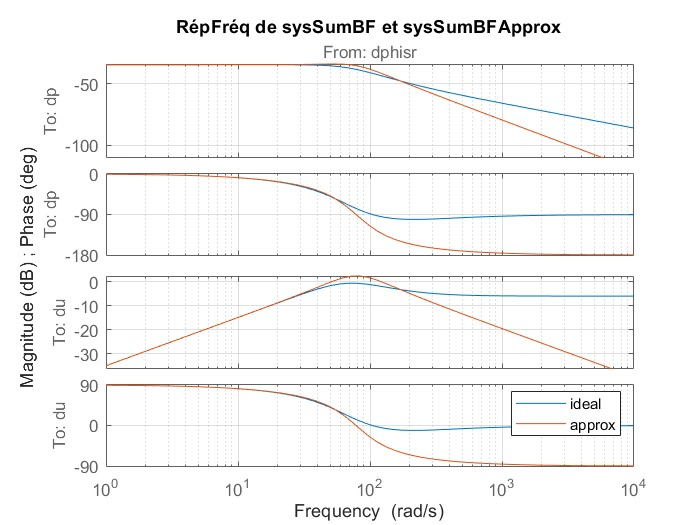
\includegraphics[width=\textwidth]{figures/repfreqsumbf_approx.jpg}
      \end{subfigure}    
      \caption{Réponses temporelles et fréquentielles 
      du système "Sum" contrôlé.
      Avec le contrôleur avec dérivée filtrée, la 
      réponse oscille un peu et est en retard.
      La réponse sur $u$ à une marge de phase de 180° et une 
      marge de gain infinie ce qui est satisfaisant.}
\end{figure}

Pour le sous-système "Dif", nous avons accéléré la dynamique avec
$\sigma = 15$

\chapter{Identification des paramètres physiques}

Nous avons rassemblé toutes les valeurs numériques dans ce 
\href{https://docs.google.com/spreadsheets/d/1PVCPAeFXgacQK3YaMxcYYtDlWB_0VT0cpRnJDznpAQc/edit?pli=1#gid=0
}{Google Sheet}.

\paragraph{Estimation de la constante de couple k}

Les équations électriques à l'équilibre s'écrivent

\begin{equation*}
    \begin{cases}
        0 = U - RI - k\Omega \\
        \tau = kI       
    \end{cases}
\end{equation*}

En se plaçant sans couple, donc sans courant, 
et en utilisant les courbes constructeurs, on calcule
$k=\frac{U}{\Omega} \, V/(rad.s^-1)$.

\begin{figure}[h]  % Placement "here"
    \centering
    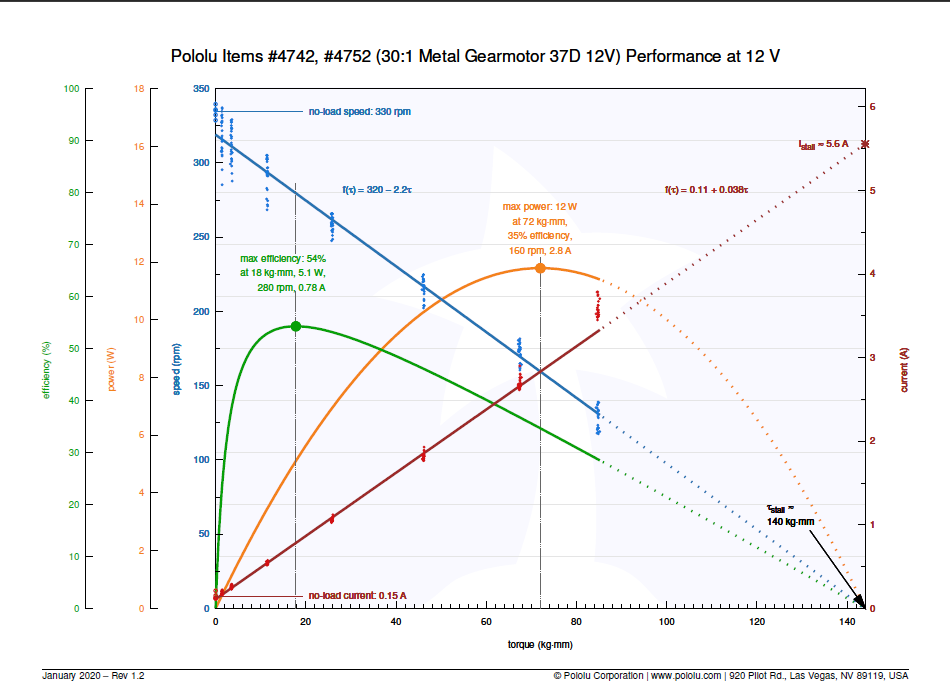
\includegraphics[width=3cm]{figures/courbes-construc.png}
    \caption{Courbes de fonctionnement fournies par Pololu.}
\end{figure}

\paragraph{Estimation des masses des pièces}
Toutes les pièces ont été pesées.

On a approximé la masse de l'arbre moteur et du rotor à la différence
entre la masse pesée du moteur, et celle donnée par la CAO.

\paragraph{Estimation des moments d'inertie}

Pour le moment d'inertie de l'unité roue + engrenage + rotor, 
notre première approche a été d'approximer la géométrie du système à celle d'un disque,
et d'utiliser la matrice d'inertie (cellule D34 du GSheet):

\begin{equation*}
    I_w(C_w) = 
    \begin{pmatrix}
        m \big(\rho^2/4 + l_w^2/2 \big) & 0 & 0 \\
        0 & m \big(\rho^2/4 + l_w^2/2 \big) & 0 \\
        0 & 0 & m \big(R^2/4 + l^2/12 \big)
    \end{pmatrix}
\end{equation*}

Comme autre approche, nous avons mesuré le temps de réponse de la 
vitesse angulaire de la roue à un échelon de 12V aux bornes du moteur.
Nous avons mesuré la sommes des positions angulaires, que nous avons filtrée 
avec un filtre passe bas, en supposant que cela ne fausse pas sensiblement le 
temps de réponse.

\begin{figure}[h]  % Placement "here"
    \centering
    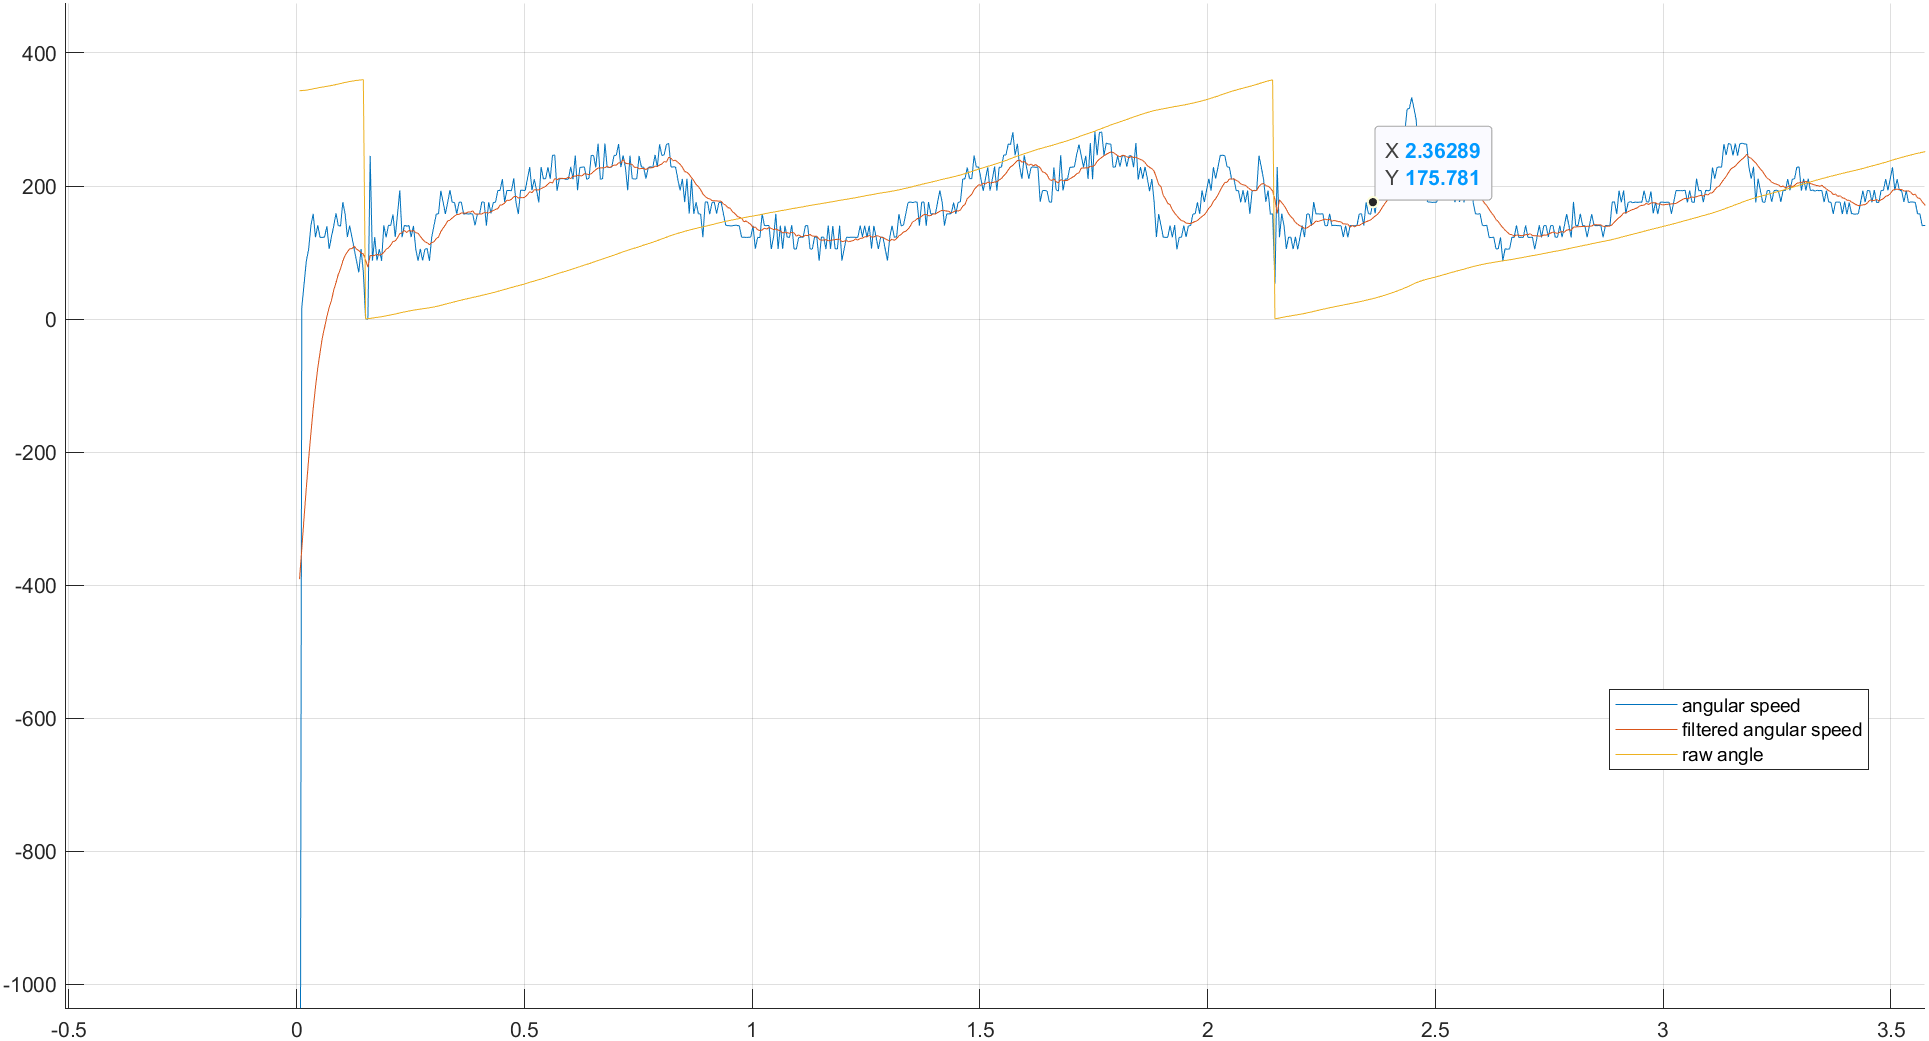
\includegraphics[width=3cm]{figures/inertie_roue.png}
    \caption{Vitesse angulaire (degrés/s) de la roue en fonction du temps (s).}
\end{figure}

Les données constructeurs fournissent une relation 
linéaire entre la vitesse angulaire et le couple d'entrée. $$\omega = a - b\tau$$

On a essayé d'exploiter le théorème du moment cinétique à l'unité roue+rotor:

$$I_w^y\dot{\omega} = \tau = \frac{a}{b} - \frac{\omega}{b}$$
$$\dot{\omega} +  \frac{\omega}{T} = \frac{a}{T} \text{  où  } T=I_w^yb$$


\paragraph{Estimation des constantes électriques}
La résistance et l'inductance interne du moteur ont été trouvées sur Internet 
\href{https://forum.pololu.com/t/mechanics-and-electrical-parameters/18153/2}{ici}.

\chapter{Implémentation du contrôleur en Arduino}
\paragraph{Structure}

Après discussion avec M. Di Meglio, le contrôleur que nous voulions implémenter en Arduino se composait de :
\begin{itemize}
\item Un contrôleur PD sur le sous-système "Sum" prenant en entrée la mesure de la somme des angles, renvoyant la somme des tensions des deux moteurs, et qui régit la vitesse en translation
\item Un contrôleur PD sur le sous-système "Diff", prenant en entrée la mesure de la distance par rapport à la ligne (donnée par le Line Follower Array), renvoyant la différence des tensions des deux moteurs, et qui régit la vitesse en rotation.
\end{itemize}
\paragraph{Contrôle de l'écart à la ligne} 

Nous avons d'abord implémenté un contrôleur P sur le sous-système "Diff" en imposant la somme des tensions (ce qui revient à imposer une vitesse longitudinale en ligne droite). Le code est disponible dans le fichier TODO: INSERER FICHIER

Après avoir effectué cette implémentation et avoir trouvé des gains satisfaisants, nous avons implémenté le contrôleur PD sur le sous-système "Diff", puis réglé les gains de ce contrôleur à partir d'observations de la performance du robot sur le circuit. Voici quelques questions qui guidaient notre réflexion :
\begin{itemize}
    \item Le robot arrive-t-il à tourner assez dans les virages ? Si non, augmenter le gain proportionnel.
    \item Le robot est-il assez nerveux ? Si non, augmenter le gain dérivé. A l'inverse si oui (visible par des oscillations très rapides), baisser le gain dérivé.
\end{itemize}

Le code correspondant est disponible dans le fichier TODO: INSERER FICHIER.

Nous nous sommes également questionnés sur l'utilité de l'implémentation d'un PID plutôt qu'un PD sur l'écart par rapport à la ligne, mais nous avons abandonné cette idée en raison de la quantification du Line Follower Array :
\begin{itemize}
    \item Avant l'implémentation, nous avions l'intuition que l'ajout d'un terme intégral n'allait pas être satisfaisant à cause de la quantification du capteur, qui est importante : il est très dur d'arriver parfaitement au "0" du Line Follower Array, même en étant sur la ligne. Il n'aurait donc pas été possible de se débarasser de l'erreur statique, même avec un terme intégral. Au contraire, ce terme rajouterait des erreurs "numériques".
    \item De brefs tests sur le circuit ont confirmé cette intuition.
\end{itemize}
% \printbibliography

\paragraph{Contrôle de la vitesse en translation}
Après avoir implémenté le contrôleur PD sur l'écart à la ligne, nous avons essayé d'implémenter le contrôle de la vitesse en translation, matérialisé par la somme des tensions des deux moteurs. Le code correspondant est disponible dans TODO:INSERER FICHIER

Néanmoins, les gains proposés par Matlab sur ce sous-système n'étaient pas satisfaisants et la performance du robot sur le circuit était moins bonne qu'en imposant une somme des tensions constante. Un réglage plus manuel des gains n'a pas donné de résultat satisfaisant non plus. Nous avons donc décidé de ne pas implémenter le contrôleur PD sur la somme des angles mesurés par les encodeurs.

Cependant, nous avons vite identifié que notre robot n'allait pas à une vitesse optimale en ligne droite, et nous nous sommes demandés comment nous pouvions améliorer ce comportement sans utiliser ce contrôleur. Nous avons opté pour une solution non-linéaire de "seuil" : 
\begin{itemize}
    \item Si l'écart à la ligne est supérieure à une certaine valeur seuil pré-définie, nous considérons que le robot est dans un virage, et nous adaptons sa vitesse en fonction en baissant la valeur de la commande de la somme des tensions des deux moteurs vers une valeur pré-définie.
    \item Sinon, nous considérons que le robot est en ligne droite et nous augmentons la valeur de la commande de la somme des tensions à une valeur pré-définie.
\end{itemize}
Le code correspondant, qui est celui utilisé lors du challenge, est disponible dans TODO:INSERER FICHIER.
\end{document}
